% Complete Section 2.3, PDF 22-25 / printed 12-15, ending before Section 2.4.
% Original Fraktur Z/B are represented by user-approved mathcal Z/B.
% block: simplicial-chain-heading page:22 type:section
\section{{Example: 单纯链复形}}\label{sec:simplicial-chain-complex}

% block: simplicial-complex-definition page:22 type:ordinary-paragraph
{链复形的一个经典例子, 也是许多术语的来源, 是与单纯复形相伴的\emph{单纯链复形}. 所谓某个 Euclidean 空间 $\mathbb R^n$ 中的 $k$ 维单纯形, 是指 $k+1$ 个点 $x_0,\ldots,x_k$ 的凸包 $f$; 这些点称为 $f$ 的顶点, 并假定它们在 $\mathbb R^n$ 中处于一般位置. $f$ 的顶点集的每个非空子集都确定一个维数 $\leq k$ 的单纯形, 称为 $f$ 的一个面. 单纯复形是 $\mathbb R^n$ 中单纯形的有限集合 $\mathcal S$, 满足 (1) 只要一个单纯形属于 $\mathcal S$, 它的每个面也都属于 $\mathcal S$; (2) 若 $f$ 和 $g$ 是 $\mathcal S$ 中的两个单纯形, 则它们的交 $f\cap g$ 或者为空, 或者同时是 $f$ 和 $g$ 的一个面. 单纯复形的底空间, 即这些单纯形的并所形成的 $\mathbb R^n$ 的子集, 可以是多面体区域, 分片平坦流形, 或更复杂的集合. 单纯复形的维数是其中所有单纯形维数的最大值; 若一个 $k$ 维单纯复形中的每个单纯形都包含在某个 $k$ 维单纯形中, 则称该单纯复形是\emph{纯的}.}

% block: oriented-simplices-figure page:23 type:figure
\begin{figure}[htbp]\centering
\includegraphics[page=23,trim=105bp 566bp 56bp 62bp,clip,width=.72\linewidth]{../input/source/Finite Element Exterior Calculus.pdf}
\caption{{维数为 1, 2 和 3 的定向单纯形.}}\label{fig:oriented-simplices}
\end{figure}

% block: pure-complex-triangulation page:23 type:ordinary-paragraph
{纯单纯复形的概念, 实质上与其底空间的剖分这一概念相同. 更准确地说, 一个由 $n$ 维单纯形组成的有限集合构成其并的一个剖分, 当且仅当这些单纯形连同它们所有维数的全部面, 构成一个纯 $n$ 维单纯复形.}

% block: simplex-orientation page:23 type:ordinary-paragraph
{可以通过选定顶点的一个次序为单纯形\emph{定向}, 其中约定: 若两个次序相差一个偶置换, 则认为它们等价. 因此, 每个维数 $k>0$ 的单纯形都有两种可能的定向. 见 Figure~\ref{fig:oriented-simplices}. 我们用 $[x_0,\ldots,x_k]$ 表示以 $x_0,\ldots,x_k$ 为顶点, 并配备由给定顶点次序确定的定向的单纯形. 固定单纯复形全部顶点集合的一个次序, 例如字典序, 就可以 (而且我们也将这样做) 为单纯复形 $\mathcal S$ 中的所有单纯形指定一个优先选用的定向. 此时, 若顶点序列 $x_0,\ldots,x_k$ 或它的某个偶置换按递增次序排列, 则称定向单纯形 $[x_0,\ldots,x_k]$ 为\emph{正定向的}.}

% block: simplicial-chain-definition page:23 type:ordinary-paragraph
{设 $\mathcal S$ 为 $\mathbb R^n$ 中的单纯复形, 用 $\Delta_k(\mathcal S)$ 表示其中 $k$ 维单纯形的集合. $k$-链是 $k$ 维定向单纯形的形式线性组合,}

% block: simplicial-chain-linear-combination page:23 type:equation
\[
c=\sum_{f\in\Delta_k(\mathcal S)}c_f f,
\]

% block: simplicial-chain-space page:23 type:ordinary-paragraph
{其中, 定向单纯形的 $-1$ 倍理解为同一个单纯形取相反定向. 我们主要考虑实系数链, 即 $c_f\in\mathbb R$. 因此, 所有 $k$-链组成的空间是维数为 $\#\Delta_k(\mathcal S)$ 的实向量空间, 记为 $C_k(\mathcal S)$, 或简记为 $C_k$. 对于 $\mathcal S$ 中任意定向 $k$-单纯形 $f=[x_0,x_1,\ldots,x_k]$, 我们将其边界 $\partial f$ 定义为如下 $(k-1)$-链:}

% block: oriented-simplex-boundary page:23 type:equation
\[
\partial[x_0,x_1,\ldots,x_k]:=\sum_{i=0}^k(-1)^i[x_0,\ldots,\widehat{x_i},\ldots,x_k],
\]

% block: boundary-incidence-matrix page:23 type:ordinary-paragraph
{其中 $x_i$ 上方的帽号表示省去该顶点. 因此, 定向 $k$-单纯形的边界 $\partial f$ 是包含在该单纯形几何边界中的各个 $k-1$ 维单纯形的形式和, 每个单纯形都配备适当的定向 (通过上式中的符号给出). 见 Figure~\ref{fig:boundaries-of-chains}. 边界算子通过线性性延拓到一般的链: $\partial c=\sum c_f\partial f$. 作为线性算子, $\partial_k$ 可以表示为一个矩阵, 即该单纯复形的\emph{定向关联矩阵}. 每个 $k$-链对应矩阵的一列, 每个 $(k-1)$-链对应矩阵的一行; 依照该 $(k-1)$-链以相同定向属于该 $k$-链的边界, 以相反定向属于其边界, 或根本不属于其边界, 相应矩阵元分别为 $1$, $-1$ 或 $0$.}

% block: boundaries-of-chains-figure page:24 type:figure
\begin{figure}[htbp]\centering
\includegraphics[page=24,trim=104bp 465bp 56bp 62bp,clip,width=.82\linewidth]{../input/source/Finite Element Exterior Calculus.pdf}
\caption{{链的边界.}}\label{fig:boundaries-of-chains}
\end{figure}

% block: homologous-cycles-figure page:24 type:figure
\begin{figure}[htbp]\centering
\includegraphics[page=24,trim=185bp 288bp 153bp 277bp,clip,width=.43\linewidth]{../input/source/Finite Element Exterior Calculus.pdf}
\caption{{属于同一个非零同调类的两个闭链.}}\label{fig:homologous-cycles}
\end{figure}

% block: simplicial-homology-betti page:24 type:ordinary-paragraph
{在这个背景下, $k$-边界链 $\mathcal B_k$ 确实是作为 $(k+1)$ 维链的边界出现的 $k$-链, 而闭链则是没有边界的链, 如 Figure~\ref{fig:boundaries-of-chains} 中最后的那个链, 它描述了一条闭曲线, 即没有端点的曲线. 不是边界的 $1$-闭链表明区域中存在贯通的孔洞. 例如, Figure~\ref{fig:homologous-cycles} 展示了两个这样的 $1$-闭链. 然而, 它们表明的是同一个孔洞, 因为它们之差是一个 $1$-边界链. 换言之, 它们代表同调群 $\mathcal H_k=\mathcal Z_k/\mathcal B_k$ 中的同一个陪集. 第 $k$ 个同调群的维数称为单纯复形 $\mathcal S$ 的第 $k$ 个 Betti 数: $b_k=\dim\mathcal H_k$. Betti 数是底空间的不变量: 它们不依赖于具体的剖分. 事实上, 它们是最简单的拓扑不变量之一, 因而也是推动代数拓扑发展的例子之一. 对二维和三维区域而言, 它们的含义如下:}

% block: betti-geometric-interpretation pages:24,25 type:ordinary-paragraph
\begin{itemize}
\item {$b_0$ 是区域的连通分支数.}
\item {$b_1$ 是贯通区域的孔洞数 (在三维情形中即为隧道数). 例如, 实心环面的 $b_1$ 等于 $1$.}
\item {对 $\mathbb R^2$ 中的任意有界区域, $b_2$ 均为零 (因为这样的区域总有边界, 因而不可能是一个闭链). 对三维区域, $b_2$ 是该区域所围空腔的数量, 例如空心球的 $b_2=1$.}
\item {对任意二维或三维区域, $b_3$ 均为零.}
\end{itemize}

% block: betti-domain-examples page:25 type:ordinary-paragraph
{一些三维区域的 Betti 数见 Figure~\ref{fig:betti-domain-examples}.}

% block: betti-domain-examples-figure page:25 type:figure
\begin{figure}[htbp]\centering
\includegraphics[page=25,trim=106bp 471bp 56bp 154bp,clip,width=.92\linewidth]{../input/source/Finite Element Exterior Calculus.pdf}
\caption{{一些 $\mathbb R^3$ 中区域的 Betti 数 $b_0,b_1,b_2,b_3$.}}\label{fig:betti-domain-examples}
\end{figure}
\clearpage
